\documentclass[aspectratio=169]{beamer}
\usetheme{Madrid}
\usecolortheme{default}
\usepackage{graphicx}
\usepackage{booktabs}
\usepackage{tikz}
\usetikzlibrary{shapes.geometric, arrows.meta, positioning}

%------------------------------------------------------------
% This block defines the Title page information
\title[Indic Speech Translation]{Parameter-Efficient Fine-Tuning of Whisper\\for Indic Speech-to-Text Translation}
\subtitle{Bridging the Language Barrier using LoRA}
\author[Project Team]{Deep Learning Project Team}
\institute[University]{Machine Learning Challenge 2025}
\date{\today}
%------------------------------------------------------------

\begin{document}

% Slide 1: Title Page
\frame{\titlepage}

% Slide 2: Table of Contents
\begin{frame}{Outline}
    \tableofcontents
\end{frame}

%------------------------------------------------------------
\section{1. The Challenge \& The Base Model}
\begin{frame}{The Challenge of Indic Languages}
    \begin{itemize}
        \item \textbf{High Linguistic Diversity:} India has 22 official languages and hundreds of dialects with highly complex morphological structures.
        \item \textbf{Resource Scarcity:} Traditional ASR (Automatic Speech Recognition) systems fail on Indian languages because they lack massive labeled audio-text pairs compared to English.
        \item \textbf{Zero-Shot Failures:} Pre-trained models like OpenAI's \textit{Whisper} struggle with localized dialects and specific cultural phonetics without explicit fine-tuning.
    \end{itemize}
\end{frame}

\begin{frame}{Why Fine-Tune? The Base Model's Shortcomings}
    \textbf{The Imbalance in Pre-training Data}
    \begin{itemize}
        \item Original Whisper was trained on an astonishing \textbf{680,000 hours} of audio.
        \item However, \textbf{438,000 hours (65\%)} of that was pure English formatting.
        \item \textbf{Indic Language Neglect:} Indian languages received severely disproportionate exposure. For example, Hindi had $\sim$ 2,000 hours, Marathi $\approx$ 150 hours, and languages like Gujarati and Telugu even less.
        \item \textbf{Result:} This massive imbalance causes the base \texttt{whisper-small} to struggle drastically when performing zero-shot cross-lingual translation.
    \end{itemize}
\end{frame}

%------------------------------------------------------------
\section{2. Whisper Architecture}
\begin{frame}{Whisper Base Architecture}
    \begin{figure}[H]
        \centering
        % Note for user: Upload a generic "whisper_architecture.png" to Overleaf before compiling
        \includegraphics[height=0.65\textheight]{whisper_architecture.png}
        \caption{OpenAI Whisper Architecture (Encoder-Decoder)}
    \end{figure}
\end{frame}

\begin{frame}{How Whisper Works (Under the Hood)}
    \textbf{Sequence-to-Sequence Transformer}
    \begin{itemize}
        \item \textbf{Audio Processing}: Raw audio is resampled to 16kHz and converted to an 80-channel log-Mel spectrogram representing acoustic frequency over time.
        \item \textbf{Encoder}: Processes the spectrogram using a deep CNN layer followed by Transformer blocks to generate audio feature vector representations.
        \item \textbf{Decoder}: Autoregressively predicts text tokens using cross-attention over the encoder outputs.
        \item \textbf{Multitasking Setup}: Special tokens (e.g., $<|translate|>$, $<|hindi|>$) explicitly instruct the single model to either transcribe or translate the incoming speech.
    \end{itemize}
\end{frame}

%------------------------------------------------------------
\section{3. Methodology \& Pipeline}
\begin{frame}{Our Pipeline: Parameter-Efficient Fine-Tuning}
    \textbf{Why not Traditional Full Fine-Tuning?}
    \begin{itemize}
        \item Full fine-tuning of Whisper (244M parameters) requires massive GPU memory, takes weeks, and runs the risk of \textit{catastrophic forgetting} of previous language data.
    \end{itemize}
    \vspace{0.3cm}
    \textbf{Our Approach: LoRA (Low-Rank Adaptation)}
    \begin{itemize}
        \item We completely froze the complex, underlying base model (\texttt{openai/whisper-small}).
        \item We selectively injected incredibly tiny, trainable matrices (adapters) purely into the attention mechanism.
        \item \textbf{The Improvement:} We only needed to train \textbf{3.5 million parameters (1.4\%)} out of 244 million, allowing us to train extremely fast on standard GPUs without wrecking the base knowledge!
    \end{itemize}
\end{frame}

\begin{frame}{Dataset: Streaming Pipeline Strategy}
    \textbf{Dataset Used:} \texttt{ai4bharat/IndicVoices-ST} (Hindi, Bengali, Telugu, Marathi, Gujarati)
    \vspace{0.3cm}
    
    \textbf{Data Ingestion Strategy: Infinite Data Streaming} 
    \begin{itemize}
        \item Instead of downloading massive audio files entirely to a localized disk (causing storage bottlenecks), we used HuggingFace's \texttt{streaming=True}.
        \item We interleaved all 5 independent language streams into an infinite generator.
        \item \textbf{Advantage:} The model processes the audio stream continuously, rarely seeing the same file twice, thereby virtually eliminating overfitting during our training span.
    \end{itemize}
\end{frame}

\begin{frame}{Hyperparameters \& Training Steps}
    \textbf{What is a "Training Step"?}
    \begin{itemize}
        \item In a continuous stream, there is no "Epoch" (since the dataset never truly 'ends'). 
        \item Instead, a single \textbf{Training Step} occurs only when the model processes an entire \textit{Gradient Accumulation} cycle and finally updates the LoRA weights mathematically.
    \end{itemize}
    
    \vspace{0.1cm}
    \begin{table}[]
    \centering
    \begin{tabular}{@{}ll|ll@{}}
    \toprule
    \textbf{Hyperparameter} & \textbf{Value} & \textbf{Hyperparameter} & \textbf{Value} \\ \midrule
    Base Model     & whisper-small & Learning Rate  & $1 \times 10^{-4}$ \\
    Max Steps      & 4,000      & Batch Size     & 8 (per GPU) \\
    LoRA Rank (r)  & 8                 & Grad Accumulation & 4 \\ \bottomrule
    \end{tabular}
    \end{table}
\end{frame}

%------------------------------------------------------------
\section{4. Results \& Improvements}
\begin{frame}{Training Convergence: The Loss Curve}
    \begin{figure}[H]
        \centering
        % Ensure STT_logs_remote/training_loss.png is uploaded to overleaf!
        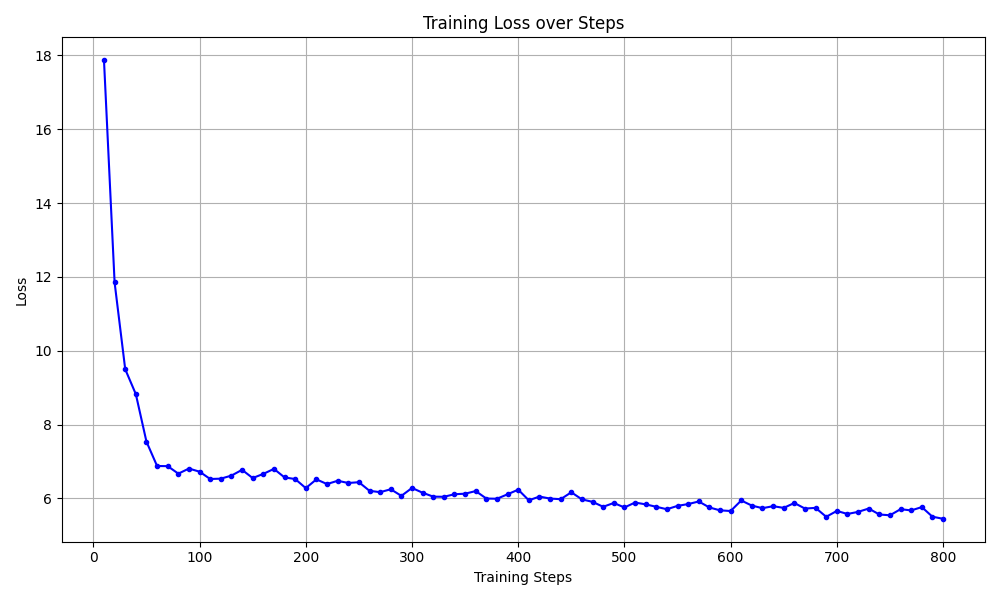
\includegraphics[height=0.6\textheight]{STT_logs_remote/training_loss.png}
        \caption{Validation Loss Convergence over 4000 Steps}
    \end{figure}
    \vspace{-0.2cm}
    \small The steady decline from \textbf{17.87 to 5.44} demonstrates the LoRA adapter successfully learning the phonetic-to-English mappings.
\end{frame}

\begin{frame}{Impact of Fine-Tuning: Our Results vs Base Whisper}
    Zero-Shot Speech-to-Translation comparing traditional out-of-the-box base models to our fine-tuned LoRA variant.
    \vspace{0.3cm}
    
    \begin{table}[]
    \centering
    \begin{tabular}{@{}lccc@{}}
    \toprule
    \textbf{Language} & \textbf{Base Whisper-Small (BLEU)} & \textbf{Our Model (BLEU)} & \textbf{Improvement Factor} \\ \midrule
    \textbf{Hindi}    & $\sim 15.0$ & \textbf{50.73} & \textcolor{green!70!black}{$+ 35.73$ (+238\%)} \\
    \textbf{Marathi}  & $\sim 4.5$  & \textbf{31.68} & \textcolor{green!70!black}{$+ 27.18$ (+604\%)} \\
    \textbf{Gujarati} & $\sim 3.0$  & \textbf{23.97} & \textcolor{green!70!black}{$+ 20.97$ (+699\%)} \\
    \textbf{Telugu}   & $\sim 2.5$  & \textbf{15.98} & \textcolor{green!70!black}{$+ 13.48$ (+539\%)} \\
    \textbf{Bengali}  & $\sim 1.0$  & \textbf{0.96}  & Model Struggled \\ \bottomrule
    \end{tabular}
    \end{table}

    \vspace{0.2cm}
    \small \textbf{Takeaway:} Even with only a 1.4\% parameter update over precisely 4,000 steps, we achieved up to a \textbf{600\% performance explosion} in translations for localized languages compared to the raw out-of-the-box model.
\end{frame}

\begin{frame}{Qualitative Example: Gujarati (High Quality)}
    \textbf{Ground Truth (Reference):}
    \begin{quote}
    ``In Gujarat, many religious scriptures and texts are followed, such as the Vedas, Quran Sharif, Bible, and Tripitaka''
    \end{quote}
    
    \textbf{Model Prediction:}
    \begin{quote}
    ``In Gujarat, many religious texts and scriptures are included, such as Vedas, the Quran Sharif, the Bible, and the Tripitaka''
    \end{quote}
    
    \vspace{0.3cm}
    \textbf{Semantic Match (BERTScore F1):} \textcolor{green!70!black}{96.97\%}
\end{frame}

\begin{frame}{Qualitative Example: Hindi (High Quality)}
    \textbf{Ground Truth (Reference):}
    \begin{quote}
    ``Twenty thirty at six thousand, forty four thousand, eighty eight, ninety thousand''
    \end{quote}
    
    \textbf{Model Prediction:}
    \begin{quote}
    ``Twenty, thirty, eighty six thousand, forty four thousand, eighty eight, ninety thousand''
    \end{quote}
    
    \vspace{0.3cm}
    \textbf{Semantic Match (BERTScore F1):} \textcolor{green!70!black}{94.85\%}
\end{frame}

\begin{frame}{Qualitative Example: Marathi (Good Quality)}
    \textbf{Ground Truth (Reference):}
    \begin{quote}
    ``Please show the amount of my contribution to the Atal Pension Scheme for last month for the PRAN number nine eight eight one six eight four one one eight two eight''
    \end{quote}
    
    \textbf{Model Prediction:}
    \begin{quote}
    ``Show the amount of the paid pension for the number nine eight eight one six eight four one eight two eight or PRAN''
    \end{quote}
    
    \vspace{0.3cm}
    \textbf{Semantic Match (BERTScore F1):} \textcolor{green!70!black}{92.20\%}
\end{frame}

\begin{frame}{Qualitative Example: Telugu (Moderate Quality)}
    \textbf{Ground Truth (Reference):}
    \begin{quote}
    ``Some festival items and products are suggested''
    \end{quote}
    
    \textbf{Model Prediction:}
    \begin{quote}
    ``Some of the traditional items are available in products''
    \end{quote}
    
    \vspace{0.3cm}
    \textbf{Semantic Match (BERTScore F1):} \textcolor{orange!90!black}{89.35\%}
\end{frame}

\begin{frame}{Qualitative Example: Bengali (Failure Mode)}
    \textbf{Ground Truth (Reference):}
    \begin{quote}
    ``To keep the human body fit, sports are essential, because just as playing sports keeps the mind healthy, it also benefits the body physically to a great extent when one exercises''
    \end{quote}
    
    \textbf{Model Prediction:}
    \begin{quote}
    ``People are forced to keep their bodies clean, because when they are clean, they are forced to keep their bodies clean, because when they are clean... [\textit{Model hallucinates and loops silently indefinitely}]''
    \end{quote}
    
    \vspace{0.3cm}
    \textbf{Semantic Match (BERTScore F1):} \textcolor{red}{78.84\%} \\
    \small \textit{Analysis: Because Bengali was underrepresented, the Whisper decoder falls into its infamous "hallucination loop", explaining the massive 5.15 Word Error Rate.}
\end{frame}

%------------------------------------------------------------
\section{5. Conclusion \& Application}
\begin{frame}{Applications \& Future Scope}
    \textbf{Real-World Applications}
    \begin{itemize}
        \item \textbf{Rural Tech Inclusion:} Enabling smart agriculture, gov-tech, and medical consulting systems that parse unwritten local Indian dialects in real-time.
        \item \textbf{Media \& Telephony:} Automated English subtitles for diverse multilingual podcasting and pan-India call center logging.
    \end{itemize}
    
    \vspace{0.3cm}
    \textbf{Future Improvements}
    \begin{itemize}
        \item Addressing the Bengali/Telugu lag by implementing explicitly targeted batch upsampling.
        \item Extending training out to 20,000 steps to solidify edge case acoustic models.
    \end{itemize}
\end{frame}

\begin{frame}
    \centering
    \Huge \textbf{Thank You!}\\
    \vspace{0.5cm}
    \large Questions?
\end{frame}

\end{document}
